\chapter{Flavour physics and CP symmetry violation}
This chapter explores the theoretical framework for the rest of the thesis.
Section \ref{sec:sm} provides a basic introduction to the Standard Model of Particle Physics and flavour physics in particular;
Section \ref{sec:discrete} delves into the inner workings of discrete symmetries in quantum physics;
Section \ref{sec:emdms} discusses the relevance of electromagnetic dipole moments of elementary particles as a test for CP violation and CPT symmetry;
finally, Section \ref{sec:lambda} introduces the main physics motivation for this thesis, the study of dipole moments of the $\Lambda^0$ baryon and the proposed measurement technique.

\section{The Standard Model of Particle Physics}
\label{sec:sm}
Ever since Democritus' philosophy of atomism, one of the driving desires behind mankind's advancements in the fields of natural science has been to reduce reality to its basic components.
While one can convincingly argue that we may never fully understand what has come to be known as the quantum world, the Standard Model of Particle Physics (Standard Model, or SM, for short) \cite{aitchinson_hey} is as close as physics has to offer to a comprehensive theory of the building blocks of matter and energy.

In addition to predicting a number of then-unknown particles discovered in later years, the Standard Model has shown remarkable consistency against high precision tests, especially in the better known electroweak sector \cite{Erler_2019}.
Despite this, it would be a mistake to call it \textit{complete}, even if only for the three fundamental forces it covers.
Many experimental evidences, some of which will be discussed in the following pages, have already opened cracks in the model, and many more may emerge in the future;
one of the recurring topics of this chapter will thus be the need for physics Beyond the Standard Model (BSM).

\subsection{Elementary particles}
\begin{figure}[t!]
	\centering
	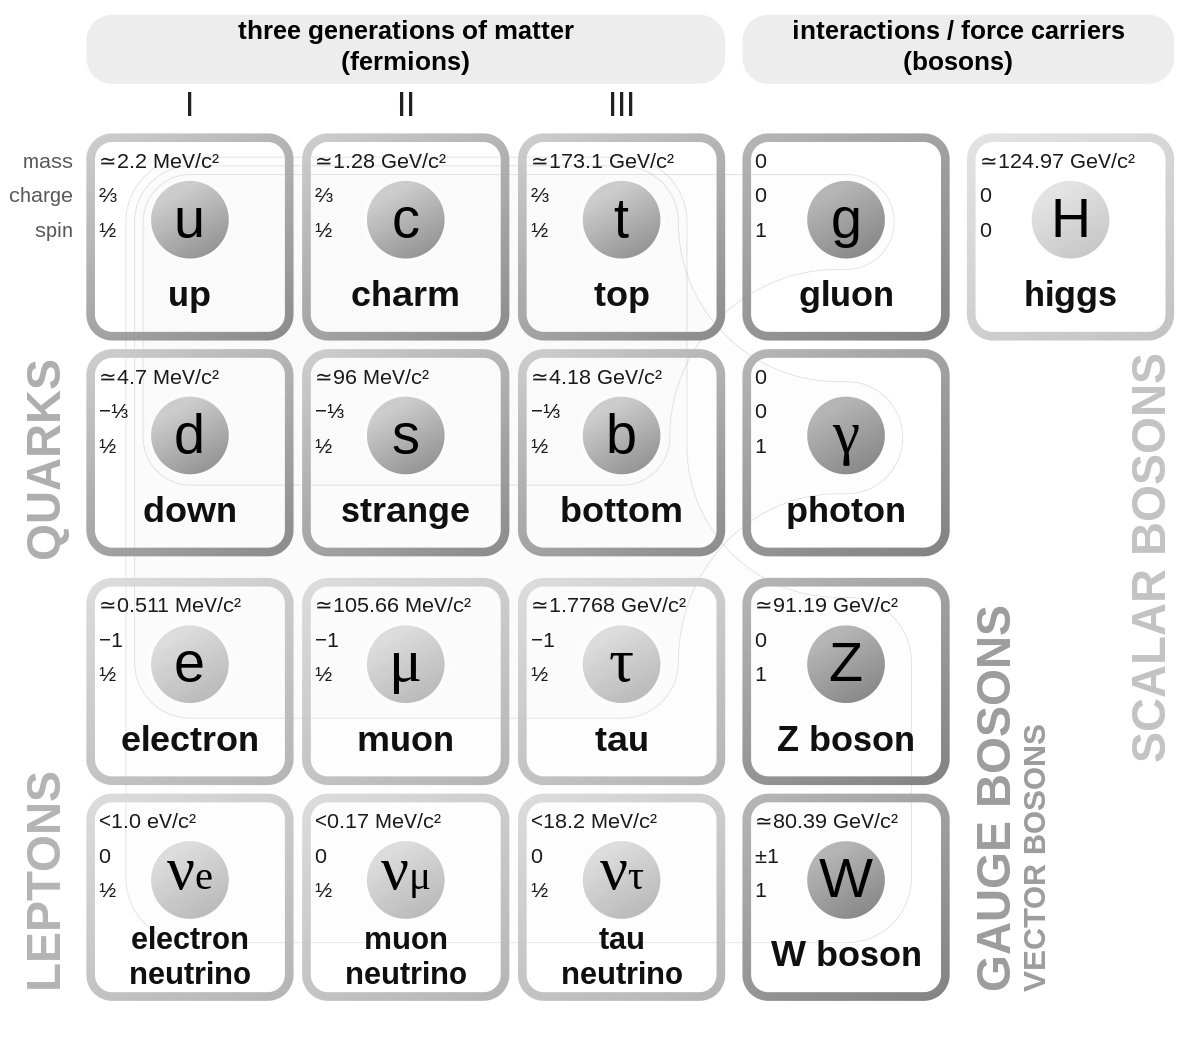
\includegraphics[width=.6\textwidth]{graphics/01-standard_model/Standard_Model_of_Elementary_Particles.png}
	\caption[Currently known Standard Model elementary particles.]{The seventeen currently known elementary particles of the Standard Model. Antiparticles are not depicted.}
	\label{fig:particle_zoo}
\end{figure}

Intuitively, a particle is said to be \textit{elementary} when no substructure can be probed. 
A century of efforts in the fields of nuclear, quantum, and high energy physics has whittled down the spectrum of matter to just seventeen unique fundamental particles, colloquially known as the \textit{particle zoo} and depicted in Figure \ref{fig:particle_zoo}.

Each particle is joined by an \textit{antimatter particle} (\textit{antiparticle} for short), a companion of opposite charge identified by the prefix \textit{anti-}, e.g. antimuon for the muon; the only exception to this naming convention is the electron, whose antiparticle, for historical reasons, is known as positron.
While often omitted for the sake of brevity, antiparticles are elementary particles in every respect, distinct from their partners (bar neutral gauge bosons and the Higgs boson, which are their own antiparticles) and related to them through the transformation of charge conjugation (see Section \ref{sec:C-symmetry}).

\subsubsection{Leptons}
Leptons are fermions (half-integer spin particles) not sensitive to the strong nuclear interaction.
There are currently six \textit{flavours} of leptons grouped in three generations: each generation comprises a \textit{charged} lepton (electron, muon, tauon) and a \textit{neutral} lepton (electron neutrino, muon neutrino, tauon neutrino).

All charged leptons have a charge of $-e$, where $e$ is the elementary positive charge, and their masses range from $\approx \SI{0.5}{MeV}$ for the electron to over $\SI{1.7}{GeV}$ for the tauon \cite{PDG}.
By contrast, as the names suggest, all neutrinos are electrically neutral and are assumed massless in the Standard Model\footnote{The observation of flavour oscillation in solar neutrinos shows that neutrinos do in fact have non-zero, albeit very small, mass \cite{SNO}.}; this implies that their only meaningful interactions happen through the weak nuclear force, which grants them their characteristic evasiveness to most particle detectors.


\subsubsection{Quarks}
Much like leptons, quarks are also fermions existing in three generations. The main difference from the former category is that quarks, besides interacting through weak and electromagnetic forces, are also susceptible to the strong nuclear forces; this allows them to bind together in composite states known as \textit{hadrons}, which are classified as \textit{baryons} (states of three quarks) and \textit{mesons} (states of one quark and one antiquark)\footnote{As recently as 2003, evidence has surfaced for the existence of exotic hadrons composed of four (\textit{tetraquarks}) \cite{tetraquark} and five quarks (\textit{pentaquarks}) \cite{pentaquark}.}.

Quarks can be classified as \textit{up-type} (up, charm and top quarks) and \textit{down-type} (down, strange and bottom quarks): up-type quarks have a fractionary charge of $+\frac{2}{3} e$, whereas down-type quarks have a charge of $-\frac{1}{3} e$. All quarks also have one of three \textit{color} charges (red, green or blue), while antiquarks similarly have one of three \textit{anti-color} charges (antired, antigreen or antiblue). A combination of all three colors/anti-colors or a combination of a color and its matching anticolor produces \textit{colorless} particles, a property shared by all observed quark composite states.

Unlike leptons, quarks are impossible to observe directly: according to the phenomenon of \textit{color confinement}, the energy of the interaction field between two color charges being pulled apart increases with their distance until it becomes high enough to create a quark-antiquark pair.
This process of \textit{fragmentation} develops many times over in such a way that the final observable state is entirely composed of colorless particles.
For this reason, high energy physics experiments such as LHCb do not detect free quarks, instead observing cone-shaped streams of hadrons known as \textit{hadronic jets}.

\subsubsection{Gauge bosons and fundamental interactions}
In quantum field theory, the interaction between two fields is implemented through the exchange of an intermediary particle known as \textit{force carrier}.
In the Standard Model all force carriers are vector (spin $1$) bosons known as \textit{gauge bosons}.
The name is owed to the \textit{gauge principle} used to introduce them: the localization of a global continuous symmetry group provides the free fermion Lagrangians with interaction terms with the proviso that one or more bosonic fields are introduced.

%The fundamental forces driving the interactions between elementary particles are introduced in the Standard Model via the so-called \textit{gauge principle}, which adds an interaction term to the free Lagrangian as a result of the localization of a global continuous symmetry group; accordingly, the related force carriers are known as \textit{gauge bosons}.

The gauge principle accounts for the implementation of three fundamental interactions along with their gauge bosons: 
the \textit{strong nuclear force} with its massless gluon, responsible for the binding of both quarks inside baryons and nucleons inside atomic nuclei; the \textit{electromagnetic force} mediated by the massless photon, the importance of which should be known from everyday life; and the \textit{weak nuclear force} with two massive $W^\pm$ and $Z$ bosons, the source of many subnuclear processes such as $\beta$ radioactivity.

The latter two forces share a unified description in the Glashow-Weinberg-Salam theory as a single \textit{electroweak interaction} and are introduced via localization of a $\text{SU(2)}_L \otimes \text{U(1)}_Y$ symmetry group, the first related to the conservation of weak isospin in left-handed chirality states and the second to the conservation of hypercharge.
Quantum chromodynamics (QCD), the theory of the strong nuclear force, is based on a separate $\text{SU(3)}_C$ symmetry acting on the three-dimensional space of color charges.

There are no gauge bosons nor gauge theories associated to the fourth known fundamental force, gravity.
Since every attempt to reconcile the general theory of relativity with quantum mechanics has failed so far, gravity is presently excluded from the Standard Model.
This doesn't affect SM predictions at the subatomic level on account of the remarkably low intensity of said force, over 30 orders of magnitude lower than the weak interaction.

\subsubsection{The Higgs boson} 
The Higgs boson is one of the latest additions to the Standard Model, being proposed in 1964 \cite{higgs1964} and observed in 2012 by the ATLAS \cite{atlasHiggs} and CMS \cite{cmsHiggs} collaborations.
Its introduction solved perhaps the most insidious SM shortcoming at the time: gauge theories, which the model was built on, only worked under the assumption that all particles involved were massless, whereas the local invariance would fall apart (\textit{gauge breaking}) when adding a free mass term.

The Higgs field accounts for mass generation of the weak bosons $W^\pm$ and $Z$ via the Brout-Englert-Higgs mechanism resulting from the spontaneous electroweak symmetry breaking;
elementary fermions also gain mass through a distinct, Yukawa-like interaction with the field.

\subsection{Flavour physics} \label{sec:flavour-physics}
A reader unfamiliar with SM terminology may find amusing the use of the word \textit{flavour} to refer to what have been so far presented as different kinds of particles altogether.
However quirky, the lexical choice highlights a defining feature: flavour, much like the degree of sweetness in a recipe, can change \cite{flavour}.

As often happens in particle physics, the rules are somewhat easier for leptons. For a given generation $\ell = (e,\mu,\tau)$, one can define a lepton family number $L_\ell$ as the difference between the number of particles and antiparticles of said generation, charged leptons and neutrinos alike:
\begin{equation}
L_\ell
\coloneqq
n(\ell^-) - n(\ell^+)
+
n(\nu_\ell) - n(\bar{\nu}_\ell).
\end{equation}
For all three generations, $L_\ell$ is conserved in every interaction except neutrino oscillations.

Quarks are not as straightforward.
A similarly defined quark flavour number, such as the so-called \textit{topness} (or \textit{truth})
\begin{equation}
T
\coloneqq
n(t) - n(\bar{t}),
\end{equation}
is preserved through EM and strong interactions, but can change when the state undergoes a weak charged interaction, i.e. a weak interaction mediated by the charged gauge bosons $W^\pm$. Weak interactions for quarks can be accurately described if we assume that the weak eigenstates $(d',s',b')$ of down-type quarks, i.e. the weak isospin doublet partners to up-type quarks, are related to the free mass eigenstates $(d,s,b)$ through a rotation:
\begin{equation}
	\begin{pmatrix}
		d' \\
		s' \\
		b'
	\end{pmatrix}
	=
	\begin{pmatrix}
		V_{ud} & V_{us} & V_{ub} \\
		V_{cd} & V_{cs} & V_{cb} \\
		V_{td} & V_{ts} & V_{tb}
	\end{pmatrix}
	\begin{pmatrix}
		d \\
		s \\
		b
	\end{pmatrix}.
	\label{eq:CKM-matrix-mixing}
\end{equation}
In this notation, the probability for a quark of flavour $i$ to change into a quark of flavour $j$ as a result of a weak charged interaction is proportional to ${\left| V_{ij} \right|}^2$.

The unitary rotation matrix is known as the Cabibbo-Kobayashi-Maskawa (CKM) matrix $V_\text{CKM}$. The moduli of its components up to the third decimal place, according to the most recent estimates \cite{PDG}, are
\begin{equation}
	\begin{pmatrix}
		\left|V_{ud}\right| & \left|V_{us}\right| & \left|V_{ub}\right| \\
		\left|V_{cd}\right| & \left|V_{cs}\right| & \left|V_{cb}\right| \\
		\left|V_{td}\right| & \left|V_{ts}\right| & \left|V_{tb}\right|
	\end{pmatrix}
	\approx 
	\begin{pmatrix}
		0.974 & 0.224 & 0.004 \\
		0.221 & 0.987 & 0.041 \\
		0.008 & 0.039 & 1.013
	\end{pmatrix}.
	\label{eq:CKM-matrix-numerical}
\end{equation}

A full definition of the CKM matrix requires four independent parameters.
Particularly useful for the following sections is the standard parameterization with three angles $\theta_{12}$, $\theta_{23}$, $\theta_{13}$, expressing the mixing between different quark generations, and a complex phase $\delta_{13}$.
Defining $s_{ik} \coloneqq \sin\theta_{ik}$ and $c_{ik} \coloneqq \cos\theta_{ik}$, $V_\text{CKM}$ can be written as
\begin{equation}
	V_\text{CKM}
	=
	\begin{pmatrix}
		c_{12} c_{13}
		&
		s_{12} c_{13}
		&
		s_{13} e^{-i\delta_{13}}
		\\
		- s_{12} c_{23} - c_{12} s_{23} s_{13} e^{i\delta_{13}}
		&
		c_{12} c_{23} - s_{12} s_{23} s_{13} e^{i\delta_{13}}
		&
		s_{23} c_{13}
		\\
		s_{12} s_{23} - c_{12} c_{23} s_{13} e^{i\delta_{13}}
		&
		-c_{12} s_{23} - s_{12} c_{23} s_{13} e^{i\delta_{13}}
		&
		c_{23} c_{13}
	\end{pmatrix}	
	\label{eq:CKM-matrix-parameterization}
\end{equation}

The phase $\delta_{13}$ is known as the CP-violating phase. To fully understand what it means and its role in particle physics, however, a digression into discrete symmetries is needed.

\section{Discrete symmetries and CP violation}
\label{sec:discrete}
In quantum mechanics, a system described by a Hamiltonian $\hat{\mathcal{H}}$ is \textit{symmetric} under a transformation $\hat{S}$ if the two operators commute, i.e.
\begin{equation}
\left[ \hat{\mathcal{H}}, \hat{S} \right] = 0.
\end{equation}
Symmetries are of great relevance in physics on account of Noether's theorem, which establishes a relationship between the \textit{continuous} symmetry of a system and a corresponding conservation law;
the emphasis is on the requirement of continuity, meaning the related transformation changes the system <<in a smooth way>>, much like a rotation does.
An example of this principle has already been presented earlier in this thesis:
the three symmetry groups employed in SM gauge theories all imply the conservation of a specific charge, be it weak isospin, hypercharge, or color.

This section will instead delve into \textit{discrete} symmetries \cite{discrete}, which do not share said <<smoothness>> property.
The absence of a Noether-like theorem for this class of transformations does not detract from their importance in physics:
as will be shown, the three symmetries we'll focus on have a remarkable influence on many fields of study.

\subsection{Parity inversion}
The \textit{parity inversion} (or simply \textit{parity}) transformation $\hat{P}$ flips the sign of the three spatial coordinates:
\begin{equation}
	\hat{P} : \begin{pmatrix}
		x \\ y \\ z
	\end{pmatrix}
	\rightarrow
	\begin{pmatrix}
		-x \\ -y \\ -z
	\end{pmatrix}.
\end{equation}
Its action on a quantum $\ket{\psi(\vec{x},t)}$ is therefore
\begin{equation}
	\hat{P} \ket{\psi(\vec{x},t)} = \ket{\psi(-\vec{x},t)}.
\end{equation}

For parity eigenstates (known as parity-defined states) a parity quantum number can be introduced;
such states may have a P-parity eigenvalue $\eta_P = +1$ (parity-even states) or $\eta_P = -1$ (parity-odd states).
Since by definition $\hat{P}^2 = \mathds{1}$, where $\mathds{1}$ is the identity operator, these are the only two allowed P-parity values.

A similarly dichotomous behaviour is observed on both scalar and vector quantities commonly used in classical physics, such as momenta and electromagnetic fields.
Parity-even scalar quantities are called \textit{true scalars} or just \textit{scalars} (e.g. energy), whereas parity-odd ones are called \textit{pseudoscalars} (e.g. helicity).
Likewise, vector quantities are either \textit{polar vectors} (e.g. angular momentum) or \textit{axial vectors} (e.g. linear momentum).

As far as is currently known, gravity, electromagnetic and strong nuclear interactions conserve parity.
The same cannot be said for the weak interaction, the P-violating properties of which were first proven in the 1956 Wu experiment on the $^{60}\text{Co}$ $\beta^-$ decay \cite{wu}. 

\subsection{Charge conjugation}
\label{sec:C-symmetry}
The transformation of \textit{charge conjugation} $\hat{C}$ changes the sign of all electric charges:
\begin{equation}
	\hat{C} : q \rightarrow -q.
\end{equation}
It should be readily apparent that $\hat{C}$ has close ties with the concept of antimatter.
The action of charge conjugation turns a quantum state into its antimatter partner, inverting the sign of all flavour quantum numbers in the process:
\begin{equation}
	\hat{C} \ket{\psi} = \ket{\bar{\psi}}.
\end{equation}
For single-particle systems, the only possible $\hat{C}$ eigenstates are particles that are their own antiparticle, like the photon, for which a C-parity $\eta_C = \pm 1$ is defined by analogy with the P-parity eigenvalue.

Unlike in the case of parity, there isn't a single breakthrough experiment credited for showing that the weak interaction is not C-symmetric:
it was known from theory that parity violation in a weak process, when observed under certain conditions, would also imply a violation of charge conjugation, with such a violation being confirmed shortly after Wu's results \cite{cviolation}.
As for the other three fundamental interactions, no evidence of C symmetry violation has surfaced so far.

\subsection{Time reversal}
Perhaps the most intuitively named of the three discrete symmetries discussed here, \textit{time reversal} $\hat{T}$ does exactly what it promises:
\begin{equation}
	\hat{T} : t \rightarrow -t .
\end{equation}
The action of time reversal on a quantum state is represented by an \textit{antiunitary} (unitary and antilinear) operator, which implies a complex conjugation on top of the time reversal itself:
\begin{equation}
	\hat{T} \ket{\psi(\vec{x},t)} = \ket{\psi^*(\vec{x},-t)}
\end{equation}
There are a number of arguments for the antiunitarity of $\hat{T}$, the most straightforward being that it prevents final states with negative energy.

Once more, gravity, strong and electromagnetic forces are T-symmetric, whereas the weak nuclear force isn't.
However, as will be explained shortly, this knowledge isn't the result of a direct experiment, instead exploiting a side effect of the CPT theorem.

\subsection{CP symmetry and violation}
\label{sec:CP-symmetry-violation}
The sequential combination of C, P and T transformations, commonly designated as CPT symmetry, plays a key role in the foundations of quantum physics.
As well as being the only combination of said transformations still observed to be a symmetry of physical laws, the \textit{CPT theorem} states that any Lorentz-invariant local quantum field theory must be CPT-symmetric.
Because a violation of the CPT symmetry would imply the collapse of the modern quantum physics framework, it is generally accepted that a T-violating process must also be a CP-violating process.
This bears an important consequence on the study of discrete symmetry violations: because of the self-evident hindrances in building a time-reversed experimental setup outside of trivial cases, every test of T violation becomes by necessity a test of CP violation.

CP symmetry is also an interesting field of study in and of itself \cite{cpvws}.
While C and P symmetries are maximally violated by the weak interaction, CP isn't;
this is exemplified by the chirally left-handed neutrino, which possesses a CP-partner (the right-handed antineutrino) despite lacking both a P-partner (the right-handed neutrino) and a C-partner (the left-handed antineutrino).

The subject of CP violation is also closely tied to another long-standing dilemma in both particle physics and cosmology: the observed asymmetry between matter and antimatter in our Universe.
A perfectly CP-symmetric system would produce a roughly equal number of particles and antiparticles, which would annihilate one another and yield an empty Universe;
our very existence implies a primordial imbalance that resulted in baryogenesis and therefore some degree of CP violation.

Since gravity, EM and strong interactions all individually conserve parity and charge conjugation, it stands to reason that they are also CP-symmetric, leaving the weak nuclear interaction as the only possible CP-violating fundamental force.
Experiments conducted over the last 50 years have found that, despite CP still being preserved in most weak processes, some select interactions show evidence of CP violation.

The first indirect discovery came in 1964 by Christenson et al. \cite{kaoncpv}, who observed the long-lived neutral kaon two-pion decay $K_L^0 \rightarrow \pi^+ \pi^-$ with a branching ratio of $\approx {10}^{-3}$ over all charged modes.
This result could only be explained by assuming that the $K_L^0$ weak eigenstate is a mixture of both $\eta_{CP}=\pm1$ eigenstates, with the ability to oscillate between the two.
A more direct evidence was found in 1999 by the KTeV collaboration at Fermilab \cite{ktevcpv} via the observation of differing decay rates in $K_{L/S}^0 \rightarrow \pi^+ \pi^-$ against $K_{L/S}^0 \rightarrow \pi^0 \pi^0$ channels, and CP violation in weak processes was definitely established in the early 2000s via studies on $B$ mesons decays conducted in so-called <<$B$-factories>> such as BaBar at SLAC \cite{babarcpv} and Belle at KEK \cite{bellecpv}.

Despite the significant number of experimental evidences collected ever since, the extent of known CP-violating processes is several orders of magnitude below what is expected from cosmological estimates.
The matter-antimatter imbalance at the time when the Universe cooled below the pair production threshold temperature can be quantified through the \textit{baryon asymmetry parameter} \cite{Canetti2012}, computed as the difference between the densities of baryons and antibaryons divided by their sum:
\begin{equation}
\eta \coloneqq \frac{n_B - n_{\bar{B}}}{n_B + n_{\bar{B}}}.
\end{equation}
While this parameter cannot be directly measured at the present time, we can approximate it by noting that almost no antimatter currently exists in the Universe ($n_{\bar{B}} \approx 0$) and almost all of the original matter will have annihilated into photons ($n_B + n_{\bar{B}} \approx n_\gamma$):
\begin{equation}
\eta \approx \frac{n_B}{n_\gamma}.
\end{equation}

Both of these quantities can be probed by studying the intergalactic medium and the cosmic microwave background, finding  $\eta_\text{obs} \approx {10}^{-10}$ \cite{Steigman2007}.
As for the Standard Model prediction, all SM sources of CP violation arise from quark mixing, more specifically from the $\delta_{13}$ complex phase mentioned in the parameterization \eqref{eq:CKM-matrix-parameterization} of the CKM matrix.
Computing the baryon asymmetry parameter with this knowledge leads to a much lower $\eta_\text{SM} \approx {10}^{-20}$ \cite{Canetti2012}.

New sources of CP violation are therefore required to match the observed value, with a promising field being the search for intrinsic electromagnetic dipole moments \cite{cpvws}.

\section{Electromagnetic dipole moments}
\label{sec:emdms}

\subsection{EDMs}
The electric dipole moment (EDM) $\vec{\delta}$ is the measure of a system's \textit{polarity}, i.e. the spatial separation of positive and negative charges within the system.
For the simplest of the relevant charge configurations, a dipole of point charges $\pm q$ separated by a distance $r$, the EDM is expressed as
\begin{equation}
	\vec{\delta} = q \vec{r},
\end{equation}
where the displacement vector $\vec{r}$ points from the negative charge to the positive one.

It's hardly a feat of imagination to theorize that a composite particle like the neutron could acquire an EDM, even if the three quarks inside it cannot be thought of as a system of charges in the classical sense.
It may be less intuitive that elementary, point-like particles such as electrons and quarks can also gain one due to quantum effects resulting in the creation and destruction of virtual particles (so-called \textit{loops} in higher order Feynman diagrams).

For a spin-$\frac{1}{2}$ particle, its EDM is written in Gaussian units as \cite{searchNewPhysics}
\begin{equation}
\vec{\delta} = d \frac{\mu_B}{2} \vec{s},
\end{equation}
where $d$ is a dimensionless quantity referred to as \textit{gyroelectric factor},
\begin{equation}
\mu_B = \frac{e\hbar}{2mc},
\label{eq:magneton}
\end{equation}
is the particle magneton, $c$ is the speed of light in a vacuum, $m$ is the particle mass and
\begin{equation}
\vec{s} = 2 \frac{\braket{\vec{S}}}{\hbar}
\label{eq:spin-polarization-vector}
\end{equation}
is the spin polarization vector, related to the average value of the spin $\vec{S}$ divided by the reduced Planck constant $\hbar$.

When the particle crosses an external electric field $\vec{E}$, its EDM will polarize by changing the direction of the spin. This introduces an energy term in the system's Hamiltonian with the form
\begin{equation}
H_\text{EDM} = - \vec{\delta} \cdot \vec{E} .
\label{eq:EDM-hamiltonian}
\end{equation}
We can now check how the term \eqref{eq:EDM-hamiltonian} behaves when acted upon by some of the discrete transformations outlined in Section \ref{sec:discrete}.
The behaviour of spin $\vec{S}$,
%and therefore
hence of the spin-related EDM $\vec{\delta}$, can easily be shown to be 
%can easily be understood by interpreting it as a particle's intrinsic angular momentum, %which in classical mechanics is written in its most basic form as
%\begin{equation}
%\vec{L} = \vec{r} \times m \frac{d\vec{r}}{dt}.
%\label{eq:angular-momentum}
%\end{equation}
%As previously explained, parity inversion operator $\hat{P}$ flips the sign of spatial coordinates.
%From the above formula it should thus be immediately apparent that $\vec{L}$, $\vec{S}$, $\vec{s}$ and $\vec{\delta}$
that of polar vectors, i.e. parity-even.
By contrast, the electric field $\vec{E}$ is an axial vector, i.e. parity-odd, which makes $H_\text{EDM}$ a parity-odd pseudoscalar:
\begin{equation}
H_\text{EDM} \xrightarrow{\hat{P}} - H_\text{EDM}.
\label{eq:EDM-hamiltonian-under-P}
\end{equation}

When considering time reversal $\hat{T}$, the situation is specular:
the EDM $\vec{\delta}$ flips its sign, whereas the electric field $\vec{E}$ remains unchanged, implying
\begin{equation}
H_\text{EDM} \xrightarrow{\hat{T}} - H_\text{EDM}.
\label{eq:EDM-hamiltonian-under-T}
\end{equation}
The above result in particular contains a crucial piece of information:
assuming the validity of the CPT theorem, a Hamiltonian containing the EDM's interaction term \eqref{eq:EDM-hamiltonian} can only be CP-symmetric if the average (or \textit{permanent}) EDM of the particle is zero.

It follows that, for a particle to have a permanent EDM, CP symmetry must be violated in some measure\footnote{This line of reasoning only applies to systems that are parity eigenstates. Water molecules are notoriously polar, but their EDMs do not violate any fundamental symmetry because the molecule's ground state is a superposition of parity-even and parity-odd eigenstates.}.
As explained in Section \ref{sec:CP-symmetry-violation}, the only known source of CP violation within the Standard Model is the complex phase $\delta_{13}$ in quark mixing, which may give a small contribution to the EDMs of point-like particles such as electrons ($\delta_e \lesssim {10}^{-40}\,e\,\text{cm}$ \cite{electronEDM}) and quarks ($\delta_q \lesssim {10}^{-34} \,e\,\text{cm}$ \cite{quarkEDM}) via beyond-tree-level diagrams. Composite particles such as baryons are accorded some leeway on account of their finite size:
the weak interaction between quarks inside the neutron, for instance, contributes to a possible EDM up to $\delta_n \lesssim {10}^{-31}\,e\,\text{cm}$ \cite{neutronEDM}.

In all cases, the predicted SM contributions are orders of magnitudes below the sensitivity reached by current generation experiments.
For all intents and purposes, the observation of a non-zero permanent EDM in a baryon would imply the discovery of a BSM source of CP violation.

\subsection{MDMs}
The magnetic dipole moment (MDM) $\vec{\mu}$ of a system can be interpreted as the measure of how intense a torque the system experiences when crossing a magnetic field $\vec{B}$:
\begin{equation}
\vec{\tau} = \vec{\mu} \times \vec{B}.
\end{equation}
Unlike the case of EDMs, the extension of MDMs from classical to quantum physics is less extreme, as long as one acknowledges the affinity between angular momentum and a particle's intrinsic spin.
A classical rotating body with charge $q$, mass $m$ and angular momentum $\vec{L}$ gains an MDM in the form
\begin{equation}
	\vec{\mu} = \frac{q}{2m} \vec{L},
\end{equation}
assuming charge and mass are identically distributed.
A very similar relation holds for a non-classical, point-like spin-$\frac{1}{2}$ particle \cite{searchNewPhysics}:
\begin{equation}
	\vec{\mu} = g \frac{\mu_B}{2} \vec{s} 
\end{equation}
Here $g$ is the dimensionless \textit{gyromagnetic factor} accounting for the transition from classical to quantum physics, whereas $\mu_B$ and $\vec{s}$ are the same particle magneton and spin polarization vector defined in equations \eqref{eq:magneton} and \eqref{eq:spin-polarization-vector} respectively.

Similary to EDMs, MDMs also induce a spin rotation when subjected to a magnetic field $\vec{B}$, introducing a Hamiltonian term
\begin{equation}
H_\text{MDM} = - \vec{\mu} \cdot \vec{B} .
\label{eq:MDM-hamiltonian}
\end{equation}
Under parity and time reversal transformations, the MDM $\vec{\mu}$ behaves in the same way as the EDM $\vec{\delta}$, both being dependent on the particle's spin $\vec{S}$ (odd under $\hat{P}$, even under $\hat{T}$).
In contrast with $\vec{E}$, however, the magnetic field $\vec{B}$ behaves in the \textit{same} way as $\vec{\mu}$, effectively cancelling out their signs when the Hamiltonian \eqref{eq:MDM-hamiltonian} is acted upon:
\begin{align}
H_\text{MDM} &\xrightarrow{\hat{P}} H_\text{MDM},
\label{eq:MDM-hamiltonian-under-P} \\
H_\text{MDM} &\xrightarrow{\hat{T}} H_\text{MDM}.
\label{eq:MDM-hamiltonian-under-T}
\end{align}

Factoring in the CPT theorem, this result entails that a non-zero intrinsic MDM for fundamental particles does not imply CP violation.
For this reason, measurements of MDMs are instead used as precision tests of the CPT theorem, since their values should not change between a particle and its antimatter partner.

\subsection{Measurement of EDMs and MDMs}
\label{sec:emdm-measurement}

%Given a particle of charge $q$ flying in a region with an \textit{homogeneous} electromagnetic field represented by the tensor $F^{\mu\nu}$, the precession of its spin 4-pseudovector $a^\mu$ is described by the Thomas-Bargmann-Michel-Telegdi (T-BMT) equation
%\begin{equation}
%	\frac{da^\mu}{d\tau} = \frac{g \mu_B}{\hbar}
%	\left[
%	F^{\mu\nu}a_\nu + (a_\alpha F^{\alpha\beta}u_\beta) \frac{u^\mu}{c^2}
%	\right]
%	- (a_\alpha \frac{q}{mc} F^{\alpha \beta}u_\beta) \frac{u^\mu}{c^2}
%\end{equation}
%$\tau$ being the proper time, $p^\mu$ being the 4-momentum vector and $u^\mu$ being the velocity vector.

For the purposes of this thesis, the measurement of EDMs and MDMs of a particle is performed by exploiting the precession of spin in an electromagnetic field \cite{EMDipoleSearch}.
In the laboratory frame, a neutral particle flying with velocity $\vec{\beta}$ through homogeneous electromagnetic fields $\vec{E}$ and $\vec{B}$ experiences a precession of the non-relativistic spin polarization vector $\vec{s}$ described by the equation
\begin{equation}
\frac{d\vec{s}}{dt} = \vec{s} \times \vec{\Omega},
\quad\quad
\vec{\Omega} \coloneqq \vec{\Omega}_\text{EDM} + \vec{\Omega}_\text{MDM}.
\end{equation}
The angular velocity vector $\vec{\Omega}$ is itself the sum of two contributions due to the respective intrinsic dipole moments of the particle:
\begin{align}
\vec{\Omega}_\text{EDM} &= \frac{d\mu_B}{\hbar}
\left(
\vec{E} - \frac{\gamma}{\gamma+1} (\vec{\beta} \cdot \vec{E})\vec{\beta} + \vec{\beta} \times \vec{B})
\right), \\
\vec{\Omega}_\text{MDM} &= \frac{g\mu_B}{\hbar}
\left(
\vec{B} - \frac{\gamma}{\gamma+1} (\vec{\beta} \cdot \vec{B})\vec{\beta} - \vec{\beta} \times \vec{E})
\right).
\end{align}
Assuming $\vec{E} = 0$, as will be the case in the experimental setup employed in this work, the angular velocity simplifies to
\begin{equation}
\vec{\Omega} = \frac{\mu_B}{\hbar}
\left[
	d\vec{\beta} \times \vec{B}
	+
	g\left(
	\vec{B} - \frac{\gamma}{\gamma+1}(\vec{\beta} \cdot \vec{B}) \vec{\beta}
	\right)
\right].
\label{eq:system_spin_precession}
\end{equation}

An analytical solution of the above system of equations is possible under the approximation that the precession of the particle spin depends only on the integrated value of the magnetic field $\vec{B}$ along the particle's flight path $l$.
In the absence of field gradients, dictated by the homogeneity requirement, such integrated field $\vec{D}$ can be written as
\begin{equation}
	\vec{D} \coloneqq \int_0^l dl' \vec{B}(\vec{r}_0 +\hat{\beta} l') \approx \braket{\vec{B}} l,
	\label{eq:integratedD}
\end{equation}
where $\hat{v}$ labels the normalized vector of $\vec{v}$.
The time evolution of the spin polarization vector $\vec{s}$ ($\vec{s}(0) = \vec{s}_0$) is
\begin{equation}
	\vec{s} \left(
		t
	\right) =
	\left(
		\vec{s}_0 \cdot \hat{\Omega}
	\right) \hat{\Omega}
	+
	\left[
		\vec{s}_0 - \left(
			\vec{s}_0 \cdot \hat{\Omega}
		\right) \hat{\Omega}
	\right]
	\cos \left(
		\left \lvert
			\vec{\Omega}
		\right\rvert t
	\right)
	+
	\left(
		\vec{s}_0 \times \hat{\Omega}
	\right)
	\sin \left(
		\left \lvert
			\vec{\Omega}
		\right\rvert t
	\right).
\label{eq:spin-precession-t_cap1}
\end{equation}

From an experimental point of view, measurement of time isn't trivial;
instead, one can efficiently measure the flight length of an unstable particle $l=\beta c t$ during its lifetime.
The equation describing the spin precession as a function of $l$ has a very similar form to \eqref{eq:spin-precession-t_cap1}:
\begin{equation}
	\vec{s} \left(
		l
	\right) =
	\left(
		\vec{s}_0 \cdot \hat{\Phi}
	\right) \hat{\Phi}
	+
	\left[
		\vec{s}_0 - \left(
			\vec{s}_0 \cdot \hat{\Phi}
		\right) \hat{\Phi}
	\right]
	\cos \left \lvert
		\vec{\Phi}
	\right\rvert
	+
	\left(
		\vec{s}_0 \times \hat{\Phi}
	\right)
	\sin \left \lvert
		\vec{\Phi}
	\right \rvert,
\label{eq:spin-precession-l_cap1}
\end{equation}
with
\begin{equation}
\vec{\Phi} = \frac{\mu_B}{|\vec{\beta}|\hbar c}
\left[
	d\vec{\beta} \times \vec{D}
	+
	g\left(
	\vec{D} - \frac{\gamma}{\gamma+1}(\vec{\beta} \cdot \vec{D}) \vec{\beta}
	\right)
\right]
\end{equation}
and $\vec{D}$ defined as in \eqref{eq:integratedD}.

Equation \eqref{eq:spin-precession-l_cap1} provides a way to measure the values of EDMs and MDMs for neutral particles by studying the change in polarization after their flight through a magnetic field.
For unstable particles, the polarization at the time of decay can be inferred in a fairly straightforward way from the angular distribution of their products.
Conversely, theoretical knowledge or measurement of the original spin polarization $\vec{s}_0$ of the particle are both far from easy tasks in a general setting.
%Thankfully, in certain instances such as the one covered in this thesis, $\vec{s}_0$ can be known by exploiting the same parity violation of weak interactions discovered in 1956 by Wu and her collaborators.

\section{Proposal of a measurement of the \texorpdfstring{$\Lambda^0$}{Lambda} electromagnetic dipole moments with the LHCb detector}
%\sectionmark{Proposal of measurement of the \texorpdfstring{$\Lambda^0$}{Lambda} electromagnetic dipole moments}
\sectionmark{Proposal of measurement of the \texorpdfstring{$\Lambda^0$}{Lambda} dipole moments at LHCb}
\label{sec:lambda}

The $\Lambda^0$ baryon, also historically known as the $\Lambda^0$ hyperon\footnote{A \textit{hyperon} is a baryon with one or more strange quarks, but no heavier quarks. The nomenclature emerged in the period following the discovery of the strange quark, when no further quarks besides the first three were known; nowadays, the term is rarely used.} and sometimes labelled only as $\Lambda$, is a spin-$\frac{1}{2}$ baryon with $(u,d,s)$ valence quarks.
As the first identified baryon beyond the two nucleons, it played a key role in the discovery and christening of the strange quark:
its mass of $\approx 1116\,\text{MeV}/c$ \cite{PDG}, the lightest among $s$-bearing baryons, meant its only viable decay channels were mediated by the flavour-changing weak interaction, giving the $\Lambda^0$ a much longer half-life than expected;
this property was dubbed \textit{strangeness}, a name later inherited by the new quark that indirectly caused it.

The $\Lambda^0$ baryon is a prime candidate to probe CP violation.
Unlike in the case of the prospective discovery of a neutron
EDM\footnote{Quantum chromodynamics allows for a CP-violating term proportional to the QCD vacuum angle $\theta$. Current measurements of the neutron EDM \cite{neutronTheta} constrain $\theta \lesssim {10}^{-10}$,
%% In realtà a me non sembra ci sia quel valore, però oh, lo citano tutti...
a fine-tuning suppression known as the \textit{strong CP problem}; nevertheless, experimental discovery of a non-zero neutron EDM could be traced back to this term and would not necessarily require the introduction of new physics.},
a non-zero $\Lambda^0$ baryon EDM could not be explained by any phenomena within the Standard Model and would therefore imply the existence of BSM physics.

\subsection{Highlights from previous measurements of the \texorpdfstring{$\Lambda^0$}{Lambda} dipole moments}

\begin{figure}[t]
	\centering
	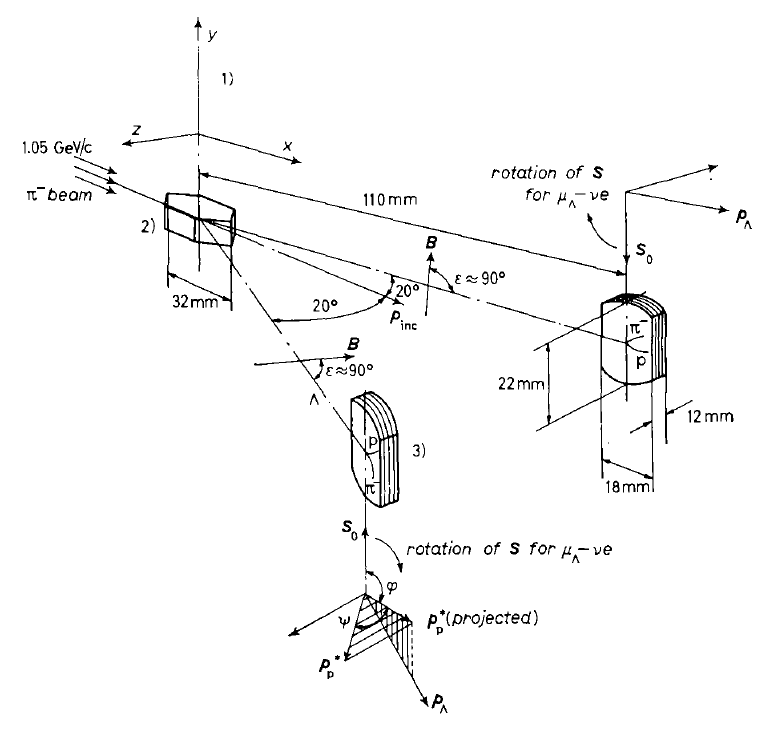
\includegraphics[width=.7\textwidth]{graphics/01-standard_model/1971_cern_emdm_setup.png}
	\caption[Experimental layout used for the 1971 $\Lambda^0$ EDM/MDM measurements.]{Experimental layout used for the 1971 $\Lambda^0$ EDM/MDM measurements \cite{1971_lambda_MDM}.}
	\label{fig:1:1971_cern_emdm_setup}
\end{figure}

Among the first meaningful measurements of the $\Lambda^0$ electromagnetic dipole moments were conducted in the early seventies at CERN near Geneva, Switzerland, by means of nuclear emulsion experiments \cite{1971_lambda_MDM} \cite{1971_lambda_EDM}.
The experimental layout is sketched in Figure \ref{fig:1:1971_cern_emdm_setup}: $\Lambda^0$ baryons are produced via reaction
\begin{equation}
	\pi^- + p \rightarrow \Lambda^0 + K^0,
\end{equation}
running a \SI{1.05}{\gev\per c} $\pi^-$ beam from the CERN Proton Synchrotron accelerator into a fixed polyethylene target.
The production cross section peaks at \SI{0.8}{\milli\barn} and the resulting $\Lambda^0$ have $\approx 100\%$ transverse polarization over a large angular production region in the reaction reference frame.
The $\Lambda^0$ angular acceptance was restricted to $18^\circ$--$22^\circ$, near the maximum production angle of $21^\circ$, to amplify the signal-to-background ratio;
this corresponds to $\Lambda^0$ with $|\vec{p}| \in \left[ \SI{500}{\mev\per c},\SI{800}{\mev\per c} \right]$.
Traversing a \SI{20}{\tesla} transverse pulsed magnetic field, $\Lambda^0$ baryons become spin-polarized as described in Section \ref{sec:emdm-measurement} before decaying into a $p\pi^-$ pair.
The final polarization direction is probed through the angular distribution of the above decay products, detected by \SI{1.2}{\milli\meter} thick Ilford K5 nuclear emulsion stacks.
The measured $\Lambda^0$ magnetic dipole moment, improving an order of magnitude over the previous world average value, was
\begin{equation}
\mu_\Lambda = \left( -0.66 \pm 0.07 \right) \mu_N,
\end{equation}
with $\mu_N$ being the nuclear magneton \cite{1971_lambda_MDM}. The $\Lambda^0$ EDM was measured at
\begin{equation}
\delta_\Lambda = \left( -5.9 \pm 2.9 \right)\times {10}^{-15}~e~\si{\centi\meter},
\end{equation}
the 95\% confidence level upper limit being found at $\delta_\Lambda \lesssim {10}^{-14}~e~\si{\centi\meter}$ \cite{1971_lambda_EDM}.

\begin{figure}[t]
	\centering
	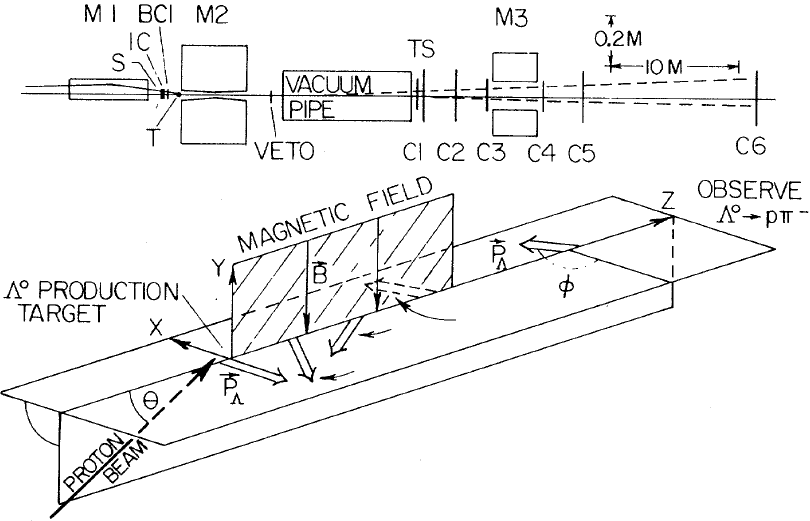
\includegraphics[width=.7\textwidth]{graphics/01-standard_model/fermilab_edm_setup.png}
	\caption[Side view of the experimental apparatus and perspective illustration of the coordinate system of the Fermilab setup for the $\Lambda^0$ EDM/MDM measurements.]{Side view of the experimental apparatus (\textit{top}) and perspective illustration of the coordinate system (\textit{bottom}) of the Fermilab setup for the $\Lambda^0$ EDM/MDM measurements \cite{PhysRevLett.41.1348}.}
	\label{fig:1:fermilab_edm_setup}
\end{figure}

These results were improved during the late seventies and early eighties with the neutral hyperon spectrometer at Fermilab in Batavia, Illinois \cite{PhysRevLett.41.1348} \cite{PhysRevD.23.814}.
Figure \ref{fig:1:fermilab_edm_setup} depicts the experimental setup: the incident \SI{300}{\gev} proton beam impacts on a beryllium target with an angle determined by the M1 upstream magnet;
outgoing particles are focused by a brass collimator and cross the M2 magnetic field, serving the dual purpose of purging the beam of charged particles and triggering the $\Lambda^0$ spin precession in the horizontal plane;
finally, the $\Lambda^0 \rightarrow p\pi^-$ decay products within a defined volumetric acceptance are detected by the C1--C6 multi-wire proportional chambers.
With a much lower $\Lambda^0$ initial polarization ($\approx 8\%$ on average) with respect to the CERN emulsion experiments, the Fermilab team was nonetheless able to best their results owing to a tenfold increase in $\Lambda^0$ statistics and precise measurement of the integrated magnetic field. The extracted value for the MDM \cite{PhysRevLett.41.1348} was
\begin{equation}
\mu_\Lambda = \left( -0.6138 \pm 0.0047 \right) \mu_N,
\end{equation}
while the EDM measurement \cite{PhysRevD.23.814} was
\begin{equation}
\delta_\Lambda = \left( -3.0 \pm 7.4 \right)\times {10}^{-17}~e~\si{\centi\meter},
\end{equation}
setting the upper limit to $\delta_\Lambda < 1.5\times{10}^{-16}~e~\si{\centi\meter}$ \cite{PDG}.
At the time of writing, this is the current best limit on the $\Lambda^0$ electric dipole moment.

\subsection{Proposal overview}
My work in this thesis is directed towards the prospective measurement of the $\Lambda^0$ baryon electromagnetic dipole moments with the LHCb experiment at the Large Hadron Collider (see Chapter \ref{cap:LHCb}), exploiting the spin precession technique outlined in Section \ref{sec:emdm-measurement}.
The unique features of the LHCb experimental setup and a careful selection of the $\Lambda^0$ production channel will allow for significant simplifications of the general equation \eqref{eq:spin-precession-l_cap1} for neutral unstable particles.

The LHCb detector is equipped with a magnetic field directed along the laboratory frame $y$ axis\footnote{The remainder of this chapter assumes the standard right-handed LHCb coordinate system, see Section \ref{info:LHCb_system}.} used for tracking purposes. Gradient field effects for the $\vec{B}$ field within the detector acceptance are negligible, being estimated at \cite{EMDipoleSearch}
\begin{equation}
\frac{\hbar}{2mc} \frac{\beta\gamma}{\gamma+1} \frac{|\nabla B|}{B} \approx 7.4 \times {10}^{-16},
\end{equation}
with $B \coloneqq |\vec{B}|$.
Assuming production near the beam collision point, the $\Lambda^0$ baryon's average mean life of $\approx 2.6 \times {10}^{-10}\, \si{\second}$ \cite{PDG} allows a sizeable number of them to traverse at least part of the LHCb magnetic field region (roughly ranging $z=\SI{2.5}{\meter}$--$\SI{7.95}{\meter}$) before decaying.
Spin precession can thus be measured, provided we know both initial and final polarization states.
% making it possible to measure both the initial and final polarizations to infer spin precession.

%As well as being a neutral particle, thereby lacking the Thomas precession effect omitted from the discussion in Section \ref{sec:emdm-measurement}, the 

\subsection{Polarization measurements}

The problem of the $\Lambda^0$ initial polarization measurement is circumvented by selecting $\Lambda^0$ produced through the weak decay of the bottom baryon $\Lambda_b^0$
\begin{equation}
\Lambda_b^0 \rightarrow J/\psi~(\rightarrow \mu^+ \mu^-)~\Lambda^0~(\rightarrow p \pi^-),
\label{eq:demonstrator_cap1}  
\end{equation}
as well as its charge-conjugate\footnote{For the sake of brevity, charge-conjugate notation will be omitted in the rest of this thesis except where relevant to the topic at hand.}
\begin{equation}
\bar{\Lambda}_b^0 \rightarrow J/\psi \, (\rightarrow \mu^+ \mu^-) \,\bar{\Lambda}^0 \, (\rightarrow \bar{p} \pi^+).
\label{eq:antidemonstrator_cap1}  
\end{equation}
Parity violation in this decay produces $\Lambda^0$ with almost $100\%$ longitudinal polarization \cite{ATLASLambdaPolarization}, meaning that the original polarization is aligned to the $\Lambda^0$ momentum in the $\Lambda_b^0$ helicity frame (see Figure \ref{fig:1:heavy-baryon-production} and related discussion).

The nature of LHCb as a forward detector implies that $\Lambda^0$ baryons will mostly fly along the laboratory frame $z$ axis, and therefore the initial polarization can be written as $\vec{s_0} = (0,0,s_0)$. Equation \eqref{eq:spin-precession-l_cap1} for the $\Lambda^0$ spin precession after the magnetic field region can thus be simplified assuming a field $\vec{B} = (0,B_y,0)$:
\begin{equation}
\vec{s} =
\begin{cases}
	s_x = -s_0 \sin\Phi\\
	s_y = -s_0 \frac{d\beta}{g} \sin\Phi \\
	s_z = s_0 \cos\Phi
\end{cases},
\label{eq:final_polarization_cap1}
\end{equation}
with
\begin{equation}
\Phi
=
\frac{D_y \mu_B}{\beta \hbar c} \sqrt{d^2 \beta^2 + g^2}
\approx
\frac{g D_y \mu_B}{\beta \hbar c}
,
\end{equation}
$\beta \coloneqq \left\lvert \vec{\beta} \right\rvert$ and
\begin{equation}
D_y \coloneqq D_y (l) = \int_0^l dl' B_y.
\end{equation}
Note from equation \eqref{eq:final_polarization_cap1} that a non-vanishing intrinsic EDM introduces a $s_y$ component to the final polarization, the MDM precession of which would otherwise be confined to the $xz$ plane.

The polarization after the magnetic field can be probed by studying the angular distribution of the $\Lambda^0 \rightarrow p\pi^-$ decay products.
%% @todo: Appendice, quando e se avrai tempo. Prima finisci i capitoli 4 e 5, poi si vede.
%(see Appendix \ref{chap:angular-distribution})
The expected angular distribution for said decay \cite{EMDipoleSearch} \cite{Richman:153636} \cite{PhysRev.108.1645} is
\begin{equation}
\frac{dN}{d\Omega'} = 1+ \alpha \vec{s} \cdot \hat{k},
\label{eq:angular_distribution_cap1}
\end{equation}
where $\Omega' \coloneqq (\theta',\phi')$ is the solid angle in the $\Lambda^0$ helicity frame (see Figure \ref{fig:1:frames_of_reference_lambda}), corresponding to the momentum direction of the proton and pointing along the unit vector
\begin{equation}
\hat{k}
=
\begin{pmatrix}
	\sin \theta' \cos \phi' \\
	\sin \theta' \sin \phi' \\
	\cos \theta'
\end{pmatrix},
\end{equation}
whereas $\alpha \approx 0.732$ \cite{PDG} is the decay asymmetry parameter.
The combined measurements of the initial polarization (from the momenta of $\Lambda^0$ produced via decays \eqref{eq:demonstrator_cap1} and \eqref{eq:antidemonstrator_cap1}) and the final polarization (from angular distribution \eqref{eq:angular_distribution_cap1}) allow for a study of $\Lambda^0$ electromagnetic dipole moments based on the single components of the precession \eqref{eq:final_polarization_cap1}.

%\begin{figure}[t]
%	\centering
%	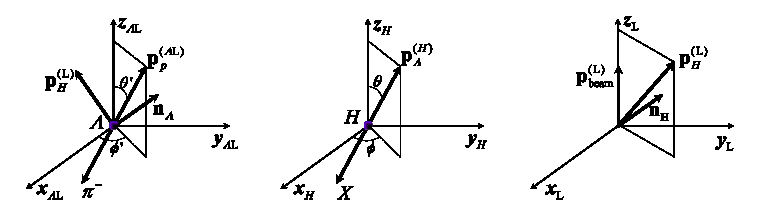
\includegraphics[scale=1]{graphics/01-standard_model/frames_of_reference.pdf}
%	\caption[Frames of reference for the $\Lambda_b^0 \rightarrow J/\psi \, (\rightarrow \mu^+ \mu^-) \,\Lambda^0 \,(\rightarrow p \pi^-)$ decay.]{Frames of reference for the $\Lambda_b^0 \rightarrow J/\psi \, (\rightarrow \mu^+ \mu^-) \,\Lambda^0 \,(\rightarrow p \pi^-)$ decay: on the \textit{left} the $\Lambda^0$ helicity frame $\text{S}_{\Lambda\text{L}}$, on the \textit{right} the laboratory frame $\text{S}_{\text{L}}$.
%	$\vec{p}_H$ is the $\Lambda_b^0$ momentum, $\vec{p}_p$ is the proton momentum (corresponding to a solid angle $(\theta',\phi')$ in the $\text{S}_{\Lambda\text{L}}$ frame), $\vec{p}_\text{beam}$ is the proton beam momentum, while $\vec{n}_\Lambda$ and $\vec{n}_H$ are the normals to the $\Lambda^0$ and $\Lambda^0_b$ production planes respectively.}
%	%\label{fig:frames_of_reference}
%\end{figure}

\begin{figure}[t]
	\centering
	\begin{subfigure}{.32\textwidth}
		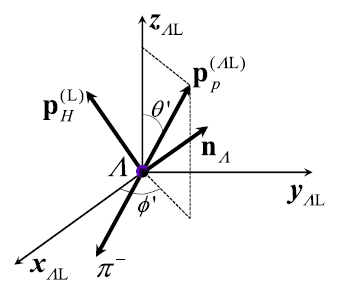
\includegraphics[width=\textwidth]{graphics/01-standard_model/helicity_frames_a.png}
		\caption{}
		\label{fig:1:frames_of_reference_lambda}
	\end{subfigure}
	\begin{subfigure}{.32\textwidth}
		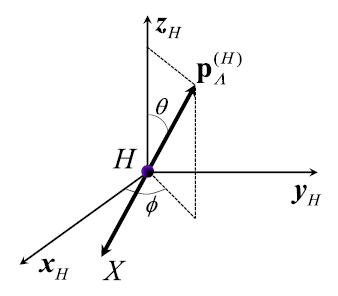
\includegraphics[width=\textwidth]{graphics/01-standard_model/helicity_frames_b.png}
		\caption{}
		\label{fig:1:frames_of_reference_heavy}
	\end{subfigure}
	\begin{subfigure}{.32\textwidth}
		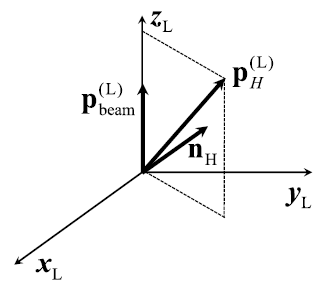
\includegraphics[width=\textwidth]{graphics/01-standard_model/helicity_frames_c.png}
		\caption{}
		\label{fig:1:frames_of_reference_lab}
	\end{subfigure}
	\caption[Frames of reference for the \demonstratorfull decay.]{Frames of reference for the \demonstratorfull decay \cite{EMDipoleSearch}: \textit{(a)} the \lz helicity frame \slambdal; \textit{(b)} the \lbz (heavy hadron) helicity frame \shad; \textit{(c)} laboratory frame \slab.
	$\vec{p}_H$ is the \lbz momentum,
	$\vec{p}_\Lambda$ is the \lz momentum (corresponding to solid angle $(\theta,\phi)$ in the $\text{S}_{\text{H}}$ frame)
	$\vec{p}_p$ is the proton momentum (corresponding to solid angle $(\theta',\phi')$ in the $\text{S}_{\Lambda\text{L}}$ frame),
	$\vec{p}_\text{beam}$ is the proton beam momentum,
	while $\vec{n}_\Lambda$ and $\vec{n}_H$ are the normals to the \lz and \lbz production planes respectively.}
	\label{fig:frames_of_reference}
\end{figure}

Deviations from this simplified treatment ought to be considered when taking into account the different relevant frames of reference, three of which are sketched in Figure \ref{fig:frames_of_reference}:
\begin{itemize}
	\item the laboratory frame \slab (Figure \ref{fig:1:frames_of_reference_lab}), with the $z$ axis along the proton beam and the $y$ axis along the vertical coordinate;
	\item the heavy hadron $\Lambda_b^0$ helicity frame \shad (Figure \ref{fig:1:frames_of_reference_heavy}), with the $z$ axis given by the $\Lambda_b^0$ momentum in \slab and the $x$ axis parallel to the normal to its production plane;
	\item the two $\Lambda^0$ helicity frames  \slambdal (Figure \ref{fig:1:frames_of_reference_lambda}) and \slambda. These are functionally the same frame of reference, the difference being that the $z$ axis is defined in the direction of the \lz momentum in \slab and \shad respectively.
\end{itemize}

The polarization given by the equation of motion derived in Section \ref{sec:emdm-measurement} refers to the comoving rest frame of the \lz (also known as the \textit{canonical frame)}, related to the $\text{S}_\text{L}$ frame by a Lorentz boost.
By contrast, Equation \eqref{eq:angular_distribution_cap1} for the angular distribution is computed with the solid angle $\Omega'$ in the particle helicity frame $\text{S}_{\Lambda\text{L}}$.
Canonical and helicity frames are related by a rotation angle, meaning that $\vec{s_0}$ is not fixed to be perpendicular to $\vec{B}$, as assumed in the solution of system  \eqref{eq:system_spin_precession}.
This effect arises in the case of \lz not directed along the $\text{S}_\text{L}$ $z$ axis and is expected to be negligible in the single-arm geometry of the LHCb detector.

\begin{figure}[t]
	\centering
	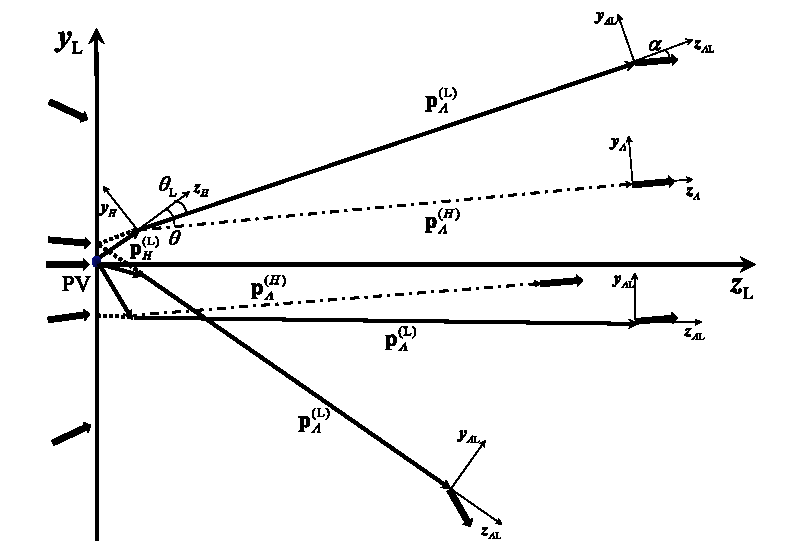
\includegraphics[scale=0.7]{graphics/01-standard_model/heavy-baryon-production.pdf}
	\caption{Sketch of the $\Lambda_b^0$ production at the primary vertex (PV) and its decay into $\Lambda^0$ in the three \shad, \slambda and \slambdal frames of reference, as seen from the \slab $yz$ plane \cite{EMDipoleSearch}. Particle momenta are represented as \textit{solid} lines for \slab, \textit{dash-dotted} lines for \shad.
	The $\Lambda^0$ polarization vector (\textit{thick arrows on the right}) is aligned to the \slambda $z$ axis and rotated by Wick angle $\alpha$ in \slambdal.
	\textit{Short-dashed} lines trace the $p_\Lambda^{(L)}$ back to the $z=z_\text{PV}$ plane, identifying the apparent production point of the $\Lambda^0$ in \slab (impact parameter).
	These points correlate with the $\Lambda^0$ helicity angle $\theta$ computed in \shad, also pictured in \slab as $\theta_\text{L}$.
	By virtue of \eqref{eq:1:wick_rotation}, this imprints a correlation between $\Lambda^0$ impact parameter and Wick rotation of its polarization vector, pictorially highlighted by the \textit{thick arrows on the left}.
	}
	\label{fig:1:heavy-baryon-production}
\end{figure}

More significant is the Wick rotation (see Figure \ref{fig:1:heavy-baryon-production}), owing to the orientation discrepancy between $\text{S}_\Lambda$ frame (where the \lz has the maximal longitudinal polarization)  and $\text{S}_{\Lambda \text{L}}$ (where the angular distribution of \lz decay products is measured).
This phenomenon introduces a dilution effect to the precession measurement: a \lz with polarization $\vec{s_0} = s_0 \hat{z}_\Lambda$ in the \slambda frame gains in the \slambdal frame a transverse component of magnitude $s_0 \sin\alpha$, where
\begin{equation}
\sin\alpha =
\frac{m_\Lambda}{m_H}
\frac{\left\lvert \vec{p}_H^{(\text{L})} \right\lvert}{\left\lvert \vec{p}_\Lambda^{(\text{L})} \right\lvert}
\sin\theta
\label{eq:1:wick_rotation}
\end{equation}
and $\theta$ is the \lz helicity angle, i.e. the angle formed by the \lz momentum in \shad with respect to the frame $z_H$ axis \cite{spinInParticlePhysics}.
As seen from Figure \ref{fig:1:heavy-baryon-production}, the helicity angle $\theta$ is related to the impact parameter with respect to the primary vertex in the \slab frame \cite{GROSNICK1990269}.
Since $\theta$ determines the magnitude of Wick angle $\alpha$, this relation can be exploited to select ensembles of $\Lambda^0$ with similar initial polarization, so that the Wick effect on the particles within a specific ensemble can be neglected.

\subsection{Closing remarks}

The LHCb tracking dipole magnet provides an integrated field $D_y \approx \pm 4 \,\si{\tesla\meter}$ \cite{LHCbDetectorPerformance}, allowing for a maximum precession angle of $\Phi_\text{max} \approx \pm \frac{\pi}{4}$ for \lz baryons traversing the entire region and reaching about 70\% of the maximum $s_y$ component in equation \eqref{eq:final_polarization_cap1}.

With the $8~\si{\per\femto\barn}$ integrated luminosity provided by the LHC Run\footnote{\textit{Run} is the conventional term for data-taking periods at LHC, see Section \ref{sec:2:lhc}.} 1 and 2 data collected with the LHCb detector and a global event reconstruction efficiency of $\varepsilon = 0.2\%$, the attainable sensitivity on the $\Lambda^0$ gyroelectric factor $d$ has been estimated at $\sigma_d \approx 1.5\times {10}^3$, to be compared with the current best limit of $1.7 \times {10}^{-2}$.
With the Run 3 projected luminosity of $\SI{50}{\per\femto\barn}$ and an efficiency of $\varepsilon = 1\%$ achievable with the upgraded LHCb trigger system (see Section \ref{sec:2:upgrade}), this limit can further be improved to $\approx 3\times {10}^{-4}$ \cite{EMDipoleSearch}.
A precision measurement of the gyromagnetic factor $g$ for $\Lambda^0$ and $\bar{\Lambda}^0$ baryons could also serve as a further precision test of the CPT theorem.


